% $Header$

\documentclass{beamer}

\mode<presentation>
{%
  \usetheme{Boadilla}
}


\usepackage[english]{babel}
\usepackage[utf8]{inputenc}
\usepackage[T1]{fontenc}

\usepackage{%
    graphicx,
    varwidth,
    animate,
    tcolorbox,
    clrscode3e,
    tikz
}
\usetikzlibrary{trees,positioning}

\graphicspath{{../../imgs/}}

% alert a whole line (especially for algorithms)
\newcommand{\alertline}{%
 \usebeamercolor[fg]{normal text}%
 \only{\usebeamercolor[fg]{alerted text}}}

% floor command
\newcommand{\floor}[1]{\left\lfloor #1 \right\rfloor}

\title[ALG25 - Lecture 3]
{Divide and Conquer \& The Master Theorem}

\subtitle
{Algorithms and Datastructures, F25, Lecture 3}

\author[Andreas H. Høeg-Petersen]
{Andreas Holck Høeg-Petersen}

\institute[AAU]{%
  Department of Computer Science\\
  Aalborg University
}

\date {\today}


\pgfdeclareimage[height=0.5cm]{university-logo}{../../imgs/aau-logo}
\logo{\pgfuseimage{university-logo}}

\AtBeginSection[]
{%
  \begin{frame}<beamer>{Outline}
    \tableofcontents[currentsection,currentsubsection]
  \end{frame}
}


\begin{document}

\begin{frame}
  \titlepage
\end{frame}

\begin{frame}{Opdateringer}{}
    \begin{itemize}
        \item Løsninger på exercises kommer på et eller andet tidspunkt
        \item Fra evaluering:
            \begin{itemize}
                \item Grupper?
                \item Andet?
            \end{itemize}
    \end{itemize}
\end{frame}


\begin{frame}{Outline}
  \tableofcontents
\end{frame}


\section{Divide and Conquer}

\begin{frame}{Divide and Conquer}{Algoritmiske teknikker}
    Divide-and-conquer er en effektiv teknik til at designe effektive
    algoritmer til at løse komplekse problemer ved at bryde dem ned i mindre
    dele. Ofte giver det en asymptotiske køretid i $\Theta(n \log n)$.

    \pause \medskip
    Metoden har overordnet set 3 skridt:

    \pause
    \begin{description}[<+->][Combine]
        \item[Divide] Del problemet op i et eller flere sub-problemer, der er
            mindre instanser af det samme problem
        \item[Conquer] Løs sub-problemerne rekursivt
        \item[Combine] Kombiner løsningerne på sub-problemerne til en løsning på
            det oprindelige problem
    \end{description}

    \pause
    Hvis problemet er småt nok (\alert{base case}), løses det uden videre.
    Ellers (\alert{recursive case}) fortsætter man rekursionen.
\end{frame}

\begin{frame}{Divide and Conquer}{Rekursion???}
    \begin{figure}[h]
        \centering
        
\includegraphics[width=0.8\textwidth]{recursion}
        \caption{Google søgning på `recursion'}
        \label{fig:recursion}
    \end{figure}

    \pause
    \begin{example}[Fibonacci-sekvensen]
        Det næste tal i Fibonacci-sekvensen er givet ved at summere de to
        foregående elementer. Den starter med 1, 1, 2, 3, 5, 8, 13, \ldots. Men
        den kan dermed også defineres rekursivt, således at det $i$'ende
        elementer er givet ved $F(i) = F(i-1) + F(i-2)$.
    \end{example}
\end{frame}

\begin{frame}{Divide and Conquer}{Algoritmisk rekursion}
    I algoritmisk forstand forstår vi en rekursion $T(n)$ således, at der for en
    tilpas stor konstant $n_0$ skal gælde følgende:

    \begin{enumerate}
        \item For alle $n < n_0$ har vi at $T(n) = \Theta(1)$ --- dvs. $T(n)$ er
            konstant
        \item For alle $n \geq n_0$ må alle stier af rekursionen ende i en
            defineret base case inden for et \alert{endeligt} antal rekursive
            kald.
    \end{enumerate}

    \pause
    I kurset her gælder det for alle rekursioner, vi ser på, men det er værd at
    have in mente, hvis I selv designer algoritmer, som gør brug af rekursion.
\end{frame}

\begin{frame}{Divide and Conquer}{Eksempler}
    I dag skal vi se på to eksempler på divide-and-conquer-algoritmer:

    \begin{itemize}
        \item Merge sort
        \item Quicksort
    \end{itemize}
\end{frame}

\section{Merge sort}

\begin{frame}{Merge sort}{Den kender I jo!}
    \begin{itemize}
        \item En af de mest berømte og benyttede sorteringsalgoritmer --- og en
            af de første til at blive implementeret i en computer (ca.\ 1945 af
            John von Neumann)
        \item Ide:
            \begin{description}
                \item[Divide] Opdel sekvensen i to lige store sub-sekvenser og kald
                    algoritmen rekursivt
                \item[Conquer] Når algoritmen modtager en sekvens med kun et element,
                    returner det trivielt sorterede element
                \item[Combine] Kombiner de sorterede sub-sekvenser, så
                    sorteringsrækkefølgen overholdes
            \end{description}
    \end{itemize}
\end{frame}

\begin{frame}{Merge sort}{Pseudo-kode del 1}
    \begin{columns}
        \column{.5\textwidth}

        \begin{itemize}[<+->]
            \small
            \item Input: en sekvens $A[1:n]$ og to \alert{indicies} $p, r$ hvor
                $1 \leq p \leq r \leq n$
            \item Ved første kald er $p=1$ og $r=n$, altså
                $\proc{Merge-Sort}(A,1,n)$
            \item I linie 3 finder vi midtpunktet mellem $p$ og $r$
            \item I linie 4 og 5 kalder vi rekursivt for den ene og anden
                halvdel af sekvensen
            \item I linie 5 kombinerer (`merger') vi de to halvdele sammen
        \end{itemize}

        \column{.5\textwidth}

        \begin{minipage}{\textwidth}
            \centering
            \begin{tcolorbox}

                \vspace{-\abovedisplayskip}
                \begin{codebox}
                    \Procname{$\proc{Merge-Sort}(A,p,r)$}
                    \li \If $p \geq r$ \Then
                        \li \Return
                    \End
                    \li $q \gets \floor{(p+r)/2}$
                    \li \proc{Merge-Sort}($A,p,q)$
                    \li \proc{Merge-Sort}($A,q+1,r$)
                    \li \proc{Merge}($A,p,q,r$)
                \end{codebox}
            \end{tcolorbox}
        \end{minipage}
        
    \end{columns}
\end{frame}

\begin{frame}{Merge sort}{Eksempel}
    
\end{frame}

\begin{frame}{Merge sort}{Merge-operationen}
    Merge-operationen er et rædselsfuldt monster i CLRS\ldots!

    \begin{figure}[h]
        \centering
        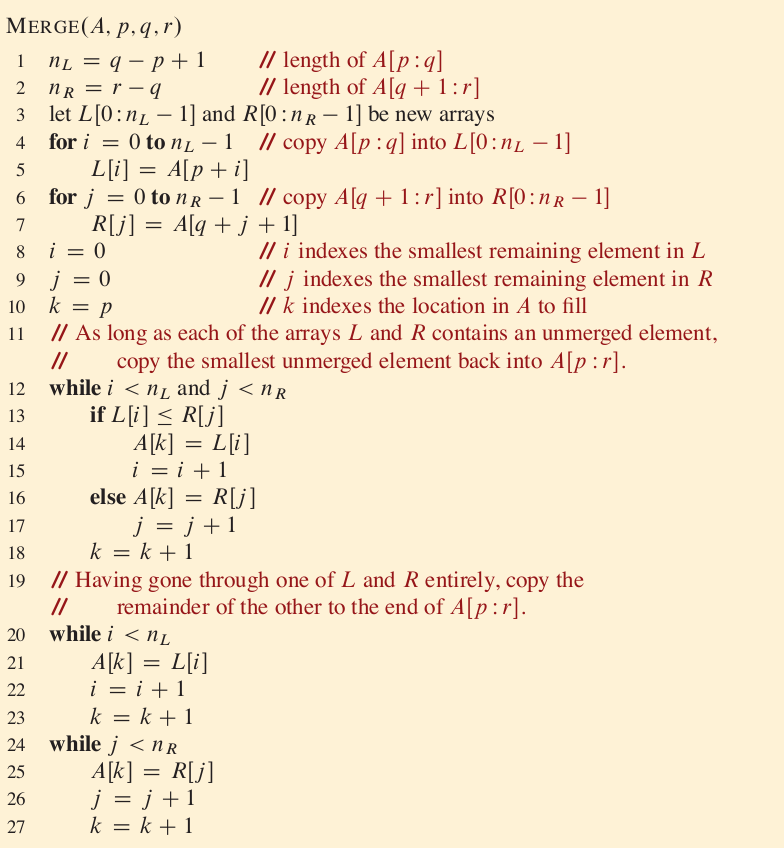
\includegraphics[width=0.45\textwidth]{merge-clrs}
        \caption{Ew!!}
        \label{fig:merge-clrs}
    \end{figure}
\end{frame}

\begin{frame}{Merge sort}{Merge-operationen}
    En lidt mere venlig version kunne se sådan her ud:

    \centering
    \begin{minipage}{.8\textwidth}
        \scriptsize
        \begin{tcolorbox}
            
            \vspace{-\abovedisplayskip}
            \begin{codebox}
                \Procname{$\proc{Merge}(A,p,q,r)$}
                \li let $B[0:r-p]$ be a new array with 0-index
                \li \For $i \gets 0$ \To $r-p$ \Do
                    \li $B[i] = A[i+p]$
                \End
                \li $i \gets 0$, $j \gets (r-q)$
                \li \For $k \gets p$ \To $r$ \Do
                    \li \If $(i + p) > q$ \Then
                        \li $A[k] \gets B[j]$
                        \li $j \gets j + 1$
                    \li \ElseIf $(j + q) > r$ \Then
                        \li $A[k] \gets B[i]$
                        \li $i \gets i + 1$
                    \li \ElseIf $B[j] < B[i]$ \Then
                        \li $A[k] \gets B[j]$
                        \li $j \gets j + 1$
                    \li \Else
                        \li $A[k] \gets B[i]$
                        \li $i \gets i + 1$
                    \End
                \End
            \end{codebox}
        \end{tcolorbox}
    \end{minipage}
\end{frame}

\begin{frame}{Merge sort}{Merge-operationen}
    Og her endda med forståelige navne:

    \centering
    \begin{minipage}{.8\textwidth}
        \scriptsize
        \begin{tcolorbox}
            
            \vspace{-\abovedisplayskip}
            \begin{codebox}
                \Procname{$\proc{Merge}(A,\id{low},\id{mid},\id{high})$}
                \li let $B[0:\id{high}-\id{low}]$ be a new array with 0-index
                \li \For $i \gets 0$ \To $\attrib{B}{length}$ \Do
                    \li $B[i] = A[i+\id{low}]$
                \End
                \zi
                \li $i \gets 0$, $j \gets (\id{high}-\id{mid})$
                \li \For $k \gets \id{low}$ \To $\id{high}$ \Do
                    \li \If $(i + \id{low}) > \id{mid}$ \Then
                        \li $A[k] \gets B[j]$
                        \li $j \gets j + 1$
                    \li \ElseIf $(j + \id{mid}) > \id{high}$ \Then
                        \li $A[k] \gets B[i]$
                        \li $i \gets i + 1$
                    \li \ElseIf $B[j] < B[i]$ \Then
                        \li $A[k] \gets B[j]$
                        \li $j \gets j + 1$
                    \li \Else
                        \li $A[k] \gets B[i]$
                        \li $i \gets i + 1$
                    \End
                \End
            \end{codebox}
        \end{tcolorbox}
    \end{minipage}
\end{frame}

\begin{frame}{Merge sort}{Merge-operationen}
    \begin{columns}
        \column{.5\textwidth}

        \centering
        \begin{minipage}{\textwidth}
            \scriptsize
            \begin{tcolorbox}
                
                \vspace{-\abovedisplayskip}
                \begin{codebox}
                    \Procname{$\proc{Merge}(A,\id{low},\id{mid},\id{high})$}
                    \li let $B[0:\id{high}-\id{low}]$ be
                    \Startalign{let $B$}
                    \>  a new array with 0-index
                    \Stopalign

                    \li \alertline<2>\For $i \gets 0$ \To $\attrib{B}{length}$ 
                    \li     \Do
                    \alertline<2>$B[i] = A[i+\id{low}]$
                            \End
                    \zi

                    \li \alertline<3>$i \gets 0$, $j \gets (\id{high}-\id{mid})$
                    \li \alertline<4>\For $k \gets \id{low}$ \To $\id{high}$ 
                    \li     \Do
                                \alertline<5>\If $(i + \id{low}) > \id{mid}$
                    \li             \Then
                                        \alertline<5>$A[k] \gets B[j]$
                    \li                 \alertline<5>$j \gets j + 1$
                    \li         \ElseIf \alertline<6>$(j + \id{mid}) > \id{high}$
                    \li             \Then
                                        \alertline<6>$A[k] \gets B[i]$
                    \li                 \alertline<6>$i \gets i + 1$
                    \li         \ElseIf \alertline<7>$B[j] < B[i]$
                    \li             \Then
                                        \alertline<7>$A[k] \gets B[j]$
                    \li                 \alertline<7>$j \gets j + 1$
                    \li         \ElseNoIf
                    \li                 \alertline<8>$A[k] \gets B[i]$
                    \li                 \alertline<8>$i \gets i + 1$
                                \End
                            \End
                \end{codebox}
            \end{tcolorbox}
        \end{minipage}

        \column{.5\textwidth}
        \begin{itemize}[<+->]
            \scriptsize
            \item Vi lader $low = p, mid = q$ og $high = r$
            \item Kopier $A[p:r]$ til $B[0:r-p]$
            \item $i$ og $j$ peger på første og anden del af $B$
            \item $k$ løber igennem alle indicies i $A[p:r]$
            \item Hvis $i$ er forbi midten, tag næste element fra $B[j:r-p]$ og
                inkrementer $j$
            \item Hvis $j$ er forbi slutningen, tag næste element fra $B[0:q-p]$
                og inkrementer $i$
            \item Hvis $B[j]$ er lavere end $B[i]$, sæt $A[k]$ til $B[j]$ og
                inkrementer $j$
            \item Ellers, sæt $A[k]$ til $B[i]$ og inkrementer $i$
            \item Vi har nu lagt elementerne fra $B$ tilbage i $A$ i sorteret
                rækkefølge!
            \item Forskellen fra CLRS er, at vi samler $L[0:n_L-1]$ og
                $R[0:n_R-1]$ i et enkelt array $B$
            \item \ldots og at vi klarer resten i et enkelt loop (fremfor 3,
                eew!)
        \end{itemize}
    \end{columns}

\end{frame}

\begin{frame}{Merge sort}{Example}
    % \begin{tikzpicture}[
    %   level distance=1.5cm,
    %   every node/.style={draw, rectangle, minimum width=1cm, minimum height=0.8cm, align=center},
    %   edge from parent path={(\tikzparentnode.south) -- (\tikzchildnode.north)}
    % ]

    %     % Root node
    %     \node {15, 7, 9, 11, 2, 8}
    %       child {~node {15, 7, 9} 
    %         child {~node {15} }
    %         child {~node {7, 9} 
    %           child {~node {7} }
    %           child {~node {9} }
    %         }
    %       }
    %       child {~node {11, 2, 8} 
    %         child {~node {11} }
    %         child {~node {2, 8} 
    %           child {~node {2} }
    %           child {~node {8} }
    %         }
    %       };

    %     % Merging process
    %     \node[below=1.5cm of {15, 7, 9}] (merge1) {Merging: 7, 9};
    %     \node[below=1.5cm of {11, 2, 8}] (merge2) {Merging: 2, 8};

    %     % Final merge
    %     \node[below=1.5cm of {merge1}] {Final Merge: 2, 7, 8, 9, 11, 15};

    % \end{tikzpicture}
\end{frame}






\section{Exercises}

\begin{frame}{Exercises!}{Yay!}
    
    \begin{figure}[h]
        \centering
        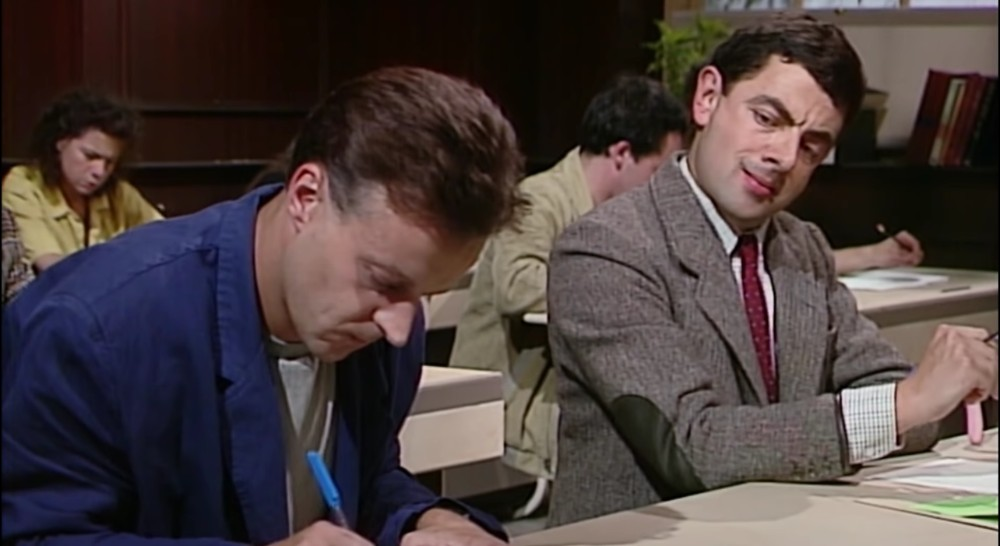
\includegraphics[width=0.8\textwidth]{exercises}
    \end{figure}
    
\end{frame}


\section{Quick sort}
\section{The Master Theorem}

\begin{frame}{Dagens temaer}{Opsummering}
    \begin{itemize}
        \item Vi har mødt vores første sorteringsalgoritme --- Insertion-Sort!
            \begin{itemize}
                \item Simpel at implementere og forstå
                \item God til næsten sorterede sekvenser
                \item Den asymptotiske worst case køretid er kvadratisk
            \end{itemize}
        \item Loop invarianter og korrekthed
            \begin{itemize}
                \item Initialization, maintenance og termination
            \end{itemize}
        \item Asymptotisk analyse og notation
            \begin{itemize}
                \item $O, \Omega, \Theta$
            \end{itemize}
    \end{itemize}
\end{frame}


\begin{frame}{Tak for i dag!}{Flere exercises..}

    Den bedste måde ikke at snyde sig selv på er lave exercises!

    \begin{figure}[h]
        \centering
        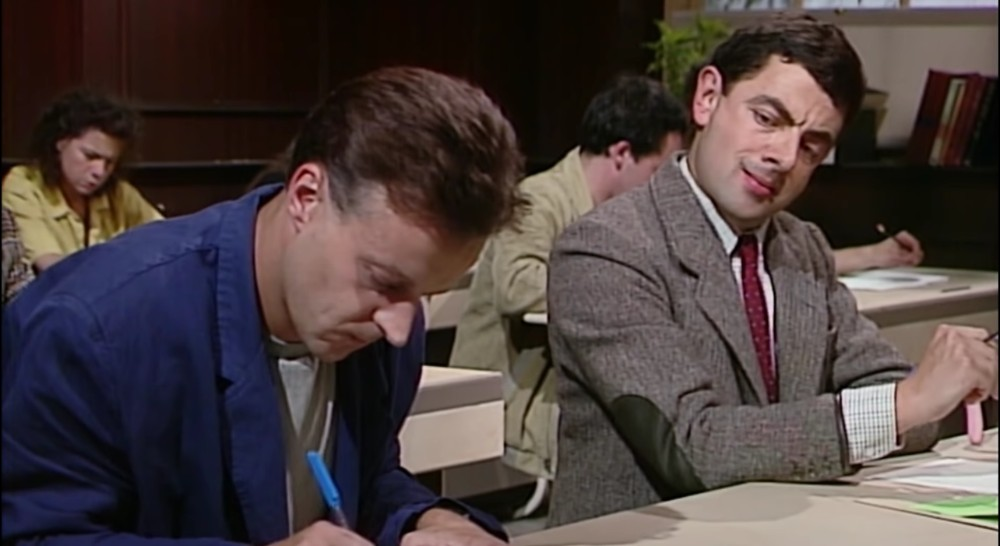
\includegraphics[width=0.8\textwidth]{exercises}
    \end{figure}
    
\end{frame}



\end{document}


